% Chapter Template

\chapter{Medical Modeling} % Main chapter title

\label{Chapter3} % Change X to a consecutive number; for referencing this chapter elsewhere, use \ref{ChapterX}
 
 %----------------------------------------------------
 
 
Digital modeling and rapid prototyping arise from the engineering need to quickly and cost-effectively design prototypes modeled using CAD software.\\
This request has led to an evolution of the software and equipment necessary to put this workflow into practice. Rapid prototyping has proved to be a useful tool, allowing to quickly evaluate the physical prototype and improve its digital design according to what it is found on the prototype, until a product that meets the required needs is obtained, iteration after iteration. \\
It was then realized that the same concept could be applied to other types of three-dimensional data, leading to the development of software to interface medical scans with rapid prototyping equipment. From the appreciation of the potential of this approach has developed the multidisciplinary field of Medical Modeling, which brings together engineers, radiologists, surgeons, designers, computer scientists and various other professionals, with the aim of using the acquired data from the patients to provide them with the highest standards of therapy \parencite{Reference1}.

\section{What can be done with patient images?}
Diagnostic images are extremely useful, both in everyday clinical practice and in research.
The digitization of acquisitions, the widespread use of computers and the variety of software available for data processing have allowed doctors to integrate imaging diagnostics into their daily activities. Diagnostic instruments are often sold by manufacturers with packages that include dedicated workstations and software. This should ensure, to the professional who buys the package, the full compatibility and integration of the workflow between the instruments purchased. \\
When using medical imaging equipment, we do not work directly with the DICOM standard, but we are dealing with the implementation of the DICOM made by the manufacturer of the instrument used. This means that compatibility is not guaranteed, but we must rely on the \emph{DICOM Conformance Statement} that the manufacturer must attach to the tool, which indicates which functions of the standard have been implemented \parencite{Reference25}. \\
Proprietary software is certainly efficient, easy to use and often has good performance, especially when used on workstations marketed by the manufacturer. At the same time, often these software are not available outside of the packages comprehensive of the diagnostic equipment, or have a high cost to be purchased by institutions on a budget or by clinicians and students who want to approach the field. In addition, the fact that software is delivered with commercial license means that its source code is not accessible, and researchers working in the field have no way of developing new functions or testing new techniques on these software. \\
For these reasons, several open-source software have been developed, which allow researchers to use the general functions of medical image processing, such as DICOM file management and image visualization, and integrate functions for advanced images analysis and processing. \\
These software cover a large part of the workflow we are going to analyze, and they provide other functionality that can be very useful when is required to perform advanced operations or create functions tailored to specific use cases.

\section{Il modello digitale}
Un modello tridimensionale è una collezione di punti, connessi a formare linee, curve, poligoni e volumi. I modelli possono essere creati con appositi software di modellazione, oppure acquisiti dal mondo reale per mezzo di dispositivi di scansione.\\
L'atto di creare un modello, la modellazione, si differenzia in \emph{modellazione organica}  e \emph{modellazione geometrica}.
\begin{wrapfigure} {R}{0.35\textwidth}
	%\centering
	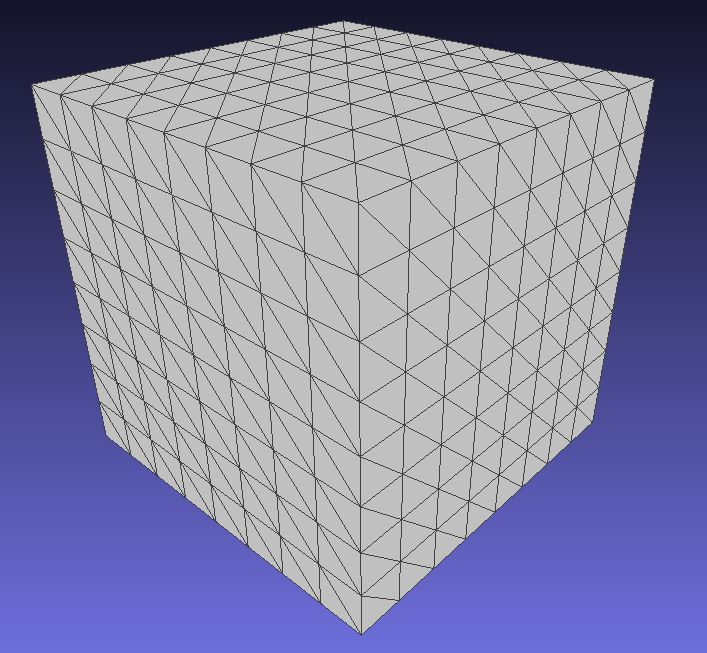
\includegraphics[width=0.35\textwidth, height=\textheight,keepaspectratio]{hr_cube_orga}
    \caption{cubo realizzato con modellazione organica; un alto numero di mesh ne aumenta la risoluzione ma ne complica la modifica.}
    \label{fig:hr_cube_orga}
\end{wrapfigure}
\paragraph{La modellazione organica} è utilizzata per realizzare geometrie naturali con forme arrotondate o irregolari, come animali, piante, pietre, esseri umani ed organi. Il modello è costituito da una superficie formata da facce poligonali, generalmente triangoli, definita \emph{mesh}. La densità dei poligoni sulla superficie rende conto della risoluzione nella rappresentazione dei dettagli. La gran parte dei modelli utilizzati in ambito medico appartengono a questa categoria, in particolar modo i modelli di parti dell'or\-ga\-ni\-smo umano.\\
Il formato più utilizzato per salvare i modelli organici è lo \textbf{.STL} (\emph{Stereolithography}, Standard Tasselation Language), che è una collezione di superfici triangolari definite dalla posizione dei vertici nello spazio e dalle normali alla superficie. Il linguaggio è stato sviluppato dalla 3d Systems per l'uso specifico con macchine per la stereolitografia, ma è ormai il linguaggio standard per modelli da utilizzare con la stampa 3D.Un consorzio di aziende operanti nel settore della modellazione tridimensionale e nella manifattura additiva è attualmente al lavoro per la creazione di un nuovo formato standard, il \textbf{.3MF} (\emph{3D Manufacturing Format}) \parencite{Reference143}.
\begin{wrapfigure} {R} {0.35\textwidth}
	%\centering
	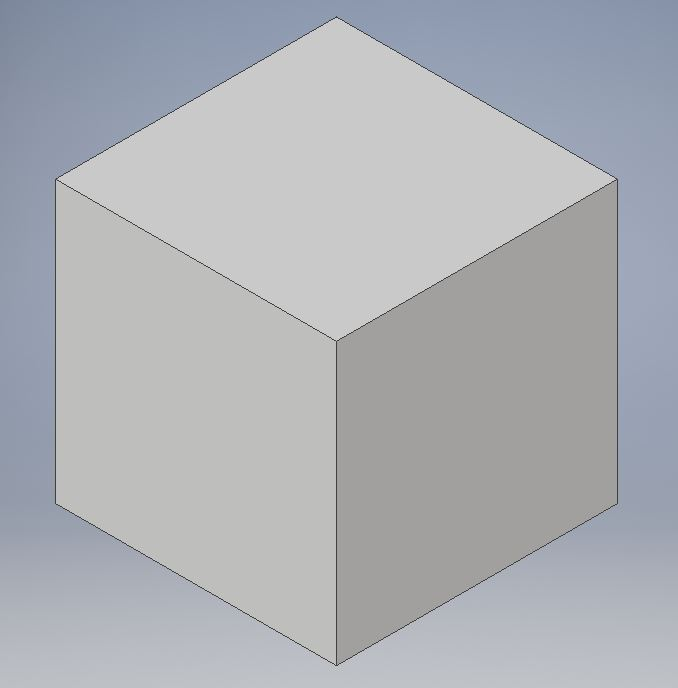
\includegraphics[width=0.35\textwidth, height=\textheight,keepaspectratio]{cube_geom}
    \caption{cubo realizzato con modellazione geometrica; il più basso numero di facce è utilizzato per descrivere il cubo.}
    \label{fig:cube_geom}
\end{wrapfigure}
\paragraph{La modellazione geometrica} è realizzata per il design di parti generalmente artificiali, dove il numero di facce del modello va ottimizzato per semplificarne progettazione, produzione ed assicurare la futura adattabilità del design. Il tipo di modellazione geometrica più diffuso è la \emph{modellazione parametrica}, adottata dai maggiori software CAD. La modellazione parametrica si basa sull'uso di primitive geometriche (linee, poligoni) le cui dimensioni sono definite ed in correlazione. La modellazione parametrica è indicata per il design di prodotti ingegneristici, protesi e guide chirurgiche. Il formato di output del modello molto spesso è dipendente dal software utilizzato, ma la maggioranza dei software di disegno parametrico permettono di esportare i modelli in .STL per le procedure di stampa 3d.

\section{3D Slicer}	
3D Slicer è un software open source per la gestione e la visualizzazione di immagini diagnostiche, realizzato da sviluppatori e ricercatori in ambito medico in un progetto supportato dal \emph{National Institute of Health} (NIH), con la collaborazione di aziende quali la \emph{Kitware Inc.} e la \emph{General Electric}, ed una community in espansione di sviluppatori volontari \parencite{Reference28}.\\
3D Slicer permette di gestire file DICOM da server \textbf{PACS} (\emph{Picture Archiving and Communication System}) e da archivi non specifici, e permette di visualizzare ed elaborare immagini in 2D, 3D e 4D (X, Y, Z e T, \emph{tempo}; ad esempio le rilevazioni con sonde ad ultrasuoni). Il software offre la capacità effettuare rendering delle immagini e di realizzare modelli per l'uso in software CAD \parencite{Reference31}.


Dal punto di vista software, Slicer ha una struttura modulare, con i moduli base (\emph{Core modules}) che forniscono le funzioni generiche di compatibilità DICOM (\emph{DICOM}) , renderizzazione (\emph{Volume rendering}) e le funzioni di trasformazione delle immagini nello spazio (\emph{Transforms}). Alcuni degli altri moduli rilevanti sono:
\begin{itemize}
\item \emph{\textbf{Filtering}}: contiene strumenti per la preparazione dell'immagine alle successive elaborazioni (\emph{preprocessing}). Le funzionalità più  usate comprendono operazioni aritmetiche, riduzione del rumore e correzione della distribuzione della densità della scansione, anche se ci sono decine di altri algoritmi che possono essere utilizzati.
\item \emph{\textbf{Registration}}: fornisce la possibilità di allineare tra loro due scansioni, utile quando devono allineare 	scanzioni diverse dello stesso paziente, oppure orientare delle scansioni per standardizzare il i dati.
\item \emph{\textbf{Segmentation}}: la segmentazione è la separazione dell'immagine in regioni più piccole in base a delle 	caratteristiche. 3D Slicer integra metodi di segmentazione sia interattiva (con input da parte 	dell'operatore) che automatica.
\item \emph{\textbf{Surface models}}: permette la creazione e la gestione di volumi di superficie da esportare per la successiva 	elaborazione in altri software
\item \emph{\textbf{Image guided Therapy}}: da la possibilità di scambiare dati in tempo reale con periferiche tra cui dispositivi 	robotici, scanner e apparati di radioterapia.
Questa funzione permette di utilizzare delle periferiche in combinazione alle immagini diagnostiche, e potrebbe essere interessante per essere usata come \emph{guida virtuale all'inserimento degli impianti} \parencite{Reference118}.
\end{itemize}
Altri moduli sono presenti, e la collezione è ampliata frequentemente con moduli realizzati dalla community o da istituzioni e aziende. Inoltre ogni utente può creare un modulo e distribuirlo come sorgente o come file binario (un file eseguibile); questa strada può usata per i pacchetti che contengono codice proprietario non libero, ma i cui autori vogliono comunque distribuire la funzionalità agli utenti \parencite{Reference28}.\\
Il software è accompagnato da delle pubblicazioni ed una documentazione che descrive le funzionalità implementate \parencite{Reference28}, \parencite{Reference29}, \parencite{Reference30}. La documentazione è il miglior riferimento per gli utenti che intendono utilizzare il software e va consultata per comprendere appieno le operazioni che ogni modulo svolge. È disponibile anche un forum su cui è possibile comunicare con utenti e sviluppatori di 3d Slicer \parencite{Reference35}.


\section{Blender} 
Blender \parencite{Reference32} è un software libero ed open-source per la computer grafica, mantenuto dalla \emph{Blender Foundation} e da una community di sviluppatori volontari. Fornisce funzionalità di base di creazione e gestione delle mesh, e funzionalità avanzate come animazioni, renderizzazioni e simulazione di effetti fisici.\\
Blender è un software che copre moltissimi aspetti della computer grafica. A guidarne l'apprendimento troviamo un'ampia documentazione delle funzionalità \parencite{Reference33}. Fondamentale risulta la community di Blender, che ha contribuito al mantenimento del software nel corso della sua evoluzione assieme alla Blender Foundation. La community è il posto dove si possono scambiare idee con esperti ed utenti del software, dove si trovano tutorial ed esempi di workflow per tutte le funzionalità di Blender \parencite{Reference34}.\\
Blender risulta molto utile per l'elaborazione dei modelli realizzati in 3d Slicer. Il software permette di modificare le mesh del modello e di compiere operazioni come la levigatura (\emph{smoothing}), la modificazione della dimensione e della risoluzione della mesh e di usare operazioni booleane tra due modelli (\emph{differenza}, \emph{unione} e \emph{intersezione}). Permette anche di eseguire rendering per creare immagini di alta qualità dei modelli.

\section{MeshLab} 
MeshLab \parencite{Reference36} è un software libero ed open source che permette la processazione avanzata delle mesh, sviluppato da studenti e ricercatori della \emph{Facoltà di Informatica dell'Università di Pisa}. Il software permette l'import/export di un'ampia quantità di file in cui si possono trovare i modelli e integra strumenti per l'ispezione della mesh e per al sua pulizia, algoritmi di remeshing e di creazione di mesh da nuvole di punti (scansioni ottiche, fotogrammetria...) e la gestione delle texture associate.\\
Questo software è utile per pulire i modelli, correggere problemi con le mesh, ridurre il numero di mesh e modificare la forma e la distribuzione delle mesh sul modello e comparare tra loro i modelli.

\section{MeshMixer} 
MeshMixer \parencite{Reference38} non è un software open-source, ma è un software gratuito rilasciato dall'azienda \emph{Autodesk}, che permette la visualizzazione e la processazione delle mesh. MeshMixer è un software con molte funzionalità, in alcuni casi sovrapponibili a quelle di software come Blender e MeshLab, provvisto di una ricca documentazione \parencite{Reference39}. \\
Questo software fornisce un'interfaccia semplice da usare, ed al contempo ottime funzionalità di manipolazione del modello e di preparazione alla stampa 3d. MeshMixer semplifica il processo di ispezione e riparazione del modello, integrando algoritmi di analisi e processazione della mesh. MeshMixer è uno strumento versatile, che può essere usato in varie parti del flusso di lavoro col modello digitale.\\
Quando si lavora con modelli semplici MeshMixer può accelerare molto la preparazione alla stampa, con strumenti che permettono di effettuare booleane tra modelli, effettuare fori e riparare aperture della mesh. Il software facilita la selezione di aree del modello da separare o su cui compiere specifiche operazioni.

\section{FreeCAD}
FreeCAD \parencite{Reference40} è un software libero ed open-source di modellazione parametrica supportato da una community di sviluppatori volontari. Il software permette di gestire la catena di produzione di un oggetto. Integra moduli per eseguire lo schizzo tecnico e realizzare il design 3d per mezzo dello schizzo o grazie alla scrittura di funzioni matematiche. Presenta moduli per l'assemblaggio di più parti e per la simulazioni fisiche, oltre che per varie altre applicazioni come la robotica o il design di barche.\\
FreeCAD è utile per la realizzazione di modelli precisi, come guide chirurgiche e protesi, ma anche parti realizzate ad hoc per la stampante 3d e per creare oggetti di utilità generale come supporti e contenitori. È un software molto versatile ed è uno strumento da conoscere per chiunque si approcci alla stampa 3D con l'intenzione di creare degli oggetti funzionali e non meramente estetici.\\
FreeCAD è supportato da una documentazione online aggiornata frequentemente \parencite{Reference41}, ed un ebook utile per comprendere le funzionalità del software, con esempi pratici anche mirati alla preparazione per la stampa 3d \parencite{Reference42}.

\section{Inventor}
Inventor \parencite{Reference43} è un software CAD professionale realizzato da \emph{Autodesk}. È tra i più avanzati software di modellazione paramentrica, ed integra tutte le funzioni di FreeCAD più molte altre. Il software viene fornito da Autodesk con un piano di abbonamento, ma per gli studenti è possibile scaricare una versione di prova della durata di 3 anni, molto utile per avere un approccio col software e testarne le caratteristiche in maniera approfondita.

\section{nTopology Element}
nTopology \parencite{Reference139} è un software commerciale di gestione di reticoli(\emph{lattice} e scaffold. È un software a pagamento ma è presente una versione free che permette di avere una panoramica delle funzioni. Il software facilita l'integrazione di modelli 3D e la loro conversione in scaffold. \\ È possibile caricare delle simulazioni fisiche in nTopology, attraverso le quali si possono ottenere degli scaffold che saranno ottimizzati rispetto ai carichi che dovranno sostenere. Utilizzeremo la versione Free di questo software per la generazione di scaffold.

\section{Cura}
Cura \parencite{Reference44} è un software open-source per la conversione in g-code (slicing) dei modelli, Il software è distribuito da Ultimaker, un produttore di stampanti 3d FDM, e supportato da una community di sviluppatori volontari. Cura è affiancato da una documentazione delle funzionalità \parencite{Reference45} e da approfonditi articoli \parencite{Reference52}.\\
Il software permette di effettuare lo slicing del modello e di regolare le opzioni di stampa. Cura permette la regolazione di molti parametri, tra cui la temperatura di stampa, l'altezza dei layer, la percentuale e la geometria di riempimento. Permette anche la creazione automatica di vari tipi di supporto, e integra la possibilità di lavorare con più di un estrusore nella stessa stampa, per effettuare stampe con più di un materiale.
Lo slicing è un processo fondamentale nel processo di stampa perché traduce il modello digitale in una serie di istruzioni. Queste vengono fornite alla stampante e risultano in una sequenza di operazioni che la essa compie per dar luogo poi ad un modello fisico, che mira ad essere l'esatta copia del modello digitale.\\
La documentazione di Cura descrive molto bene i vari parametri di stampa, perciò verranno qui brevemente descritti i parametri principali e ne saranno analizzate le implicazioni pratiche.

\subsection{Quality}
Il menù \emph{\textbf{Quality}} contiene parametri per regolare l'altezza del layer e l'ampiezza della linea di materiale estruso. Ridurre il valore di queste voci da luogo ad un aumento di qualità, perché potranno essere ricostruiti dettagli più piccoli. La scelta di questi parametri non è però arbitraria, ma si basa su delle caratteristiche della stampante.\\
L'altezza del layer (\emph{layer height}) dipende dalla risoluzione del movimento dell'estrusore sull'asse Z, che a sua volta dipende dagli step/mm, in base a meccanica di movimento e interpolazione degli step (microstep). Ad esempio, una trasmissione a vite con passo 8mm, stepper da 1,8/step e microstep 16x, fa al massimo step da 0,04 mm sull'asse Z, il che si traduce in una risoluzione massima di 0,04mm sull'asse Z, con altezza del layer che va impostata in multipli di 0,04. Diminuire l'altezza del layer permette di riprodurre particolari più piccoli e di avere una finitura di superficie con un aspetto più levigato, ma aumenta anche il tempo di stampa, perché serviranno più layer per riprodurre il modello.
Impostare l'altezza del primo layer (\emph{Initial layer height}) con un valore più alto rispetto ai successivi da in genere una migliore adesione dell'oggetto al letto di stampa, perché un flusso di materiale più abbondante al primo strato aiuta a compensare un piano di stampa non perfettamente orizzontale.\\
L'ampiezza del layer (\emph{layer width}) dipende dal diametro dell'ugello (\emph{nozzle}) utilizzato, con ugelli più piccoli che aumentano la rappresentazione dei dettagli, ed ugelli grandi che riducono i tempi di stampa; questi si trovano attualmente in diametri che vanno dagli 0,15 mm ad oltre 1 mm. L'ampiezza va impostata su un valore vicino a quello dell'ugello, mantenendo un range di libertà per ottimizzare il risultato di stampa. Impostare un valore poco più basso del diametro effettivo può aumentare la qualità di stampa, ma va valutato di volta in volta; inoltre una ampiezza minore aumenta il tempo di stampa, perché più linee verranno usate per costituire il modello. Il valore può essere aumentato per compensare una eventuale usura dell'ugello, ma è un rimedio temporaneo ed è preferibile sostituire l'ugello usurato con uno nuovo.\\

\subsection{Shell}
Il menù \emph{\textbf{Shell}} permette di regolare i parametri delle pareti del modello (shell: guscio). Possiamo regolare in maniera indipendente lo spessore della superfici, del tetto e del pavimento del modello. Uno spessore maggiore darà una maggiore resistenza al modello ed una maggiore resistenza al passaggio dei fluidi (\emph{leaking}) che posso essere fatti passare al suo interno. Sono presenti anche vari parametri riguardo alla compensazione dell'espansione o della retrazione del materiale di stampa e per regolare in maniera fine la stampa della superficie del modello.

\subsection{Infill}
L'\emph{\textbf{infill}} è il riempimento del modello, quello che si trova all'interno della superficie i cui parametri abbiamo spiegato prima. La quantità di infill può essere impostata in percentuale, con 0\% che indica l'assenza di infill e 100\% che indica il completo riempimento del volume dell'oggetto. Sono disponibili diversi \emph{pattern} di infill, alcuni veloci come \emph{Lines} o \emph{Grid}, altri più lenti ma con migliori capacita di assorbimento delle forze, ad esempio \emph{Cubic subdivision}, mentre altri ancora utili alla stampa di oggetti deformabili, come \emph{Concentric} e \emph{Cross}.\\
L'infill da resistenza all'oggetto e funge da supporto per gli strati superiori del modello. La quantità di infill va regolata in base alle condizioni meccaniche in cui l'infill dovrà operare. Un modello che subisce sollecitazioni durante l'uso dovrà avere un infill alto e con una geometria adatta, mentre un modello da esposizione può essere realizzato con poco infill, in modo da risparmiare materiale e accelerare la stampa.
Il menù infill contiene diversi parametri che è possibile regolare, tra questi la possibilità di settare manualmente l'angolazione di alcuni pattern (\emph{Infill Line Direction}). La regolazione manuale dell'angolo delle linee di infill è un metodo veloce in cui si può eseguire il design di semplici scaffold tridimensionali \parencite{Reference138}.

\begin{figure}[h]
    \centering
    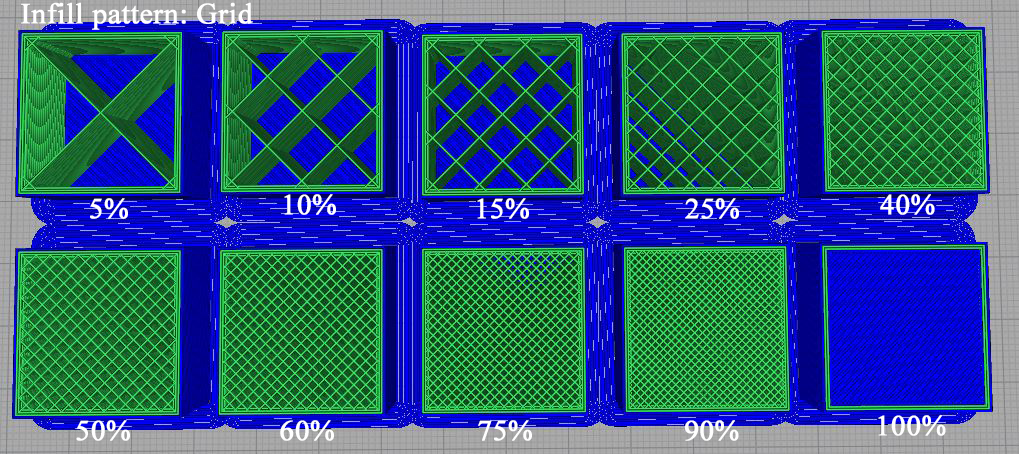
\includegraphics[width=\textwidth,height=\textheight,keepaspectratio]{numbers_grid_infillDens}
    \caption{\emph{\textbf{Infill pattern}}: \emph{Grid}; da sinistra in alto, progressivo aumento di \emph{\textbf{Infill density}}.}
    \label{fig:numbers_grid_infillDens}
\end{figure}
	

\subsection{Material}
Il menù \emph{\textbf{Material}} contiene i parametri per regolare le temperature e il processo di estrusione.
È possibile da qui regolare la temperatura di stampa (\emph{printing temperature}) e la temperatura del piano di stampa riscaldato (\emph{build plate temperature}); si può settare in maniera indipendente la temperatura del primo layer rispetto a quella dei layer successivi. Una temperatura più alta al primo layer favorisce l'adesione di questo al piano, perché il materiale estruso è meno viscoso e si spalma meglio sulla superficie. Il piano riscaldato facilita anch'esso l'adesione, che è comunque correlata al materiale di cui il piano è fatto.\\
Il flusso (\emph{flow}) si regola in percentuale e va regolato per evitare eccessi o carenze di materiale estruso durante la stampa. Un metodo di regolazione consiste nell'osservare la superficie dell'oggetto stampato per vedere se sono presenti spazi o eccessi tra i layer, e variare la percentuale di flow fino a che non appare uniforme. Un altro metodo consiste nello stampare un cubo senza tetto, infill 0\% e con le pareti spesse una linea (in \emph{shell}-->\emph{wall line count} = 1), e con un calibro misurare se la parete è effettivamente spessa lo stesso valore impostato in \emph{shell}-->\emph{wall line width}.
Questo metodo empirico può dare una indicazione sulla discrepanza tra il valore cercato ed il valore reale. La relazione tra lo spessore della parete e il valore del flow non è comunque lineare, perché la quantità di estrusione è influenzata da parametri come velocità di stampa, diametro effettivo del filamento e temperatura di stampa.\\
Un parametro importante è la retrazione (\emph{retraction}). La retrazione è la distanza di cui il filamento viene tirato indietro dall'estrusore ogni volta che finisce un segmento di stampa; questo movimento serve a ridurre la pressione all'interno dell'ugello ed a limitare la fuoriuscita di materiale fuso durante tragitti in cui non c'è stampa (\emph{oozing}). I valori di distanza di retrazione e velocità di retrazione vanno regolati con appositi test, assieme a temperatura di estrusione e \emph{jerk}.

\subsection{Speed}
\begin{wrapfigure} {R} {0.37\textwidth}
	%\centering
	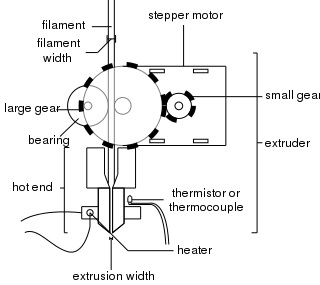
\includegraphics[width=0.37\textwidth, height=\textheight,keepaspectratio]{estrusore_diag}
    \caption{Estrusore diretto (direct extruder)}
    \label{fig:estrusore_diag}
\end{wrapfigure}
Il menù \emph{\textbf{Speed}} permette di impostare la velocità di stampa. Si può regolare la velocità di stampa della shell e dell'infill in maniera separata, la velocità dei movimenti senza stampa e le accelerazioni durante le varie fasi di stampa.
Il \emph{jerk} è un parametro che gestisce il massimo cambio di velocità istantanea dell'estrusore; un valore basso addolcisce le accelerazioni e decelerazioni mentre un valore alto le rende più brusche. L'effetto del jerk è più evidente lavorando a velocità elevate \parencite{Reference53}.\\
La velocità di stampa va regolata secondo le possibilità della stampante. Stampe veloci sono generalmente meno precise di stampe lente, e per oggetti in cui si richiede precisione dovrebbe essere preferita un velocità più bassa. Stampe veloci causano vibrazioni della struttura e instabilità nel flusso di materiale, per cui vanno fatte stampe di prova per valutare come la stampante si comporta alle varie velocità.\\

\begin{wrapfigure} {R} {0.5\textwidth}
	%\centering
	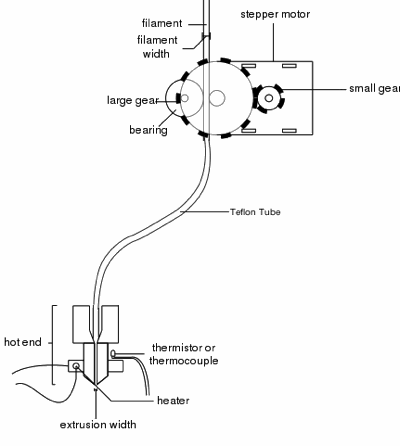
\includegraphics[width=0.5\textwidth, height=\textheight,keepaspectratio]{bowden}
    \caption{Estrusore Bowden (Bowden extruder)}
    \label{fig:bowden}
\end{wrapfigure}
La velocità dipende anche dall'inerzia delle parti in movimento, per cui avere poche parti leggere in movimento sarebbe di aiuto per aumentare la velocità nelle operazioni stampa.
Il sistema di estrusione del filamento nelle stampanti FDM è costituito essenzialmente da un estrusore ed un hotend. L'estrusore è la parte che spinge il filamento nell'hotend, il quale riscaldandosi sciogliendo il filamento, che fuoriesce dall'ugello sotto la spinta dell'estrusore. Spesso nelle stampanti FDM cartesiane è usata una estrusione definita \emph{diretta}, che consiste nell'estrusore collegato all'hotend, entrambi in movimento sugli assi.\\
Per alleggerire la massa in movimento, e quindi l'inerzia, è possibile utilizzare una configurazione di estrusione definita \emph{bowden} \parencite{Reference54}, \parencite{Reference55}, dove l'estrusore è lontano dall'hotend. La diminuzione nella massa in movimento, dovuta alla dissociazione tra il processo di estrusione e quello di fusione del materiale, permette di stampare a velocità più alte senza degradare eccessivamente la qualità di stampa. Nell'estrusione bowden il filamento va dall'estrusore all'hotend generalmente passando attraverso un tubo in \emph{Teflon} (PTFE), e compie un tragitto decisamente più lungo rispetto all'estrusione diretta; ciò causa una minore responsività del filamento nelle fasi di estrusione e retrazione. Questo effetto può essere compensato in Cura regolando i parametri di priming e retrazione del filamento.

\subsection{Travel}
Il menù \emph{\textbf{Travel}} contiene opzioni per gestire i movimenti della stampante durante i movimenti senza estrusione. L'opzione \emph{Combing Mode} restringe il movimento dell'ugello all'area di stampa del modello per ridurre la necessità di retrazione. Questo parametro può essere sempre attivo, attivo solo nell'infill o spento. Da regolare in base al modello che si intende stampare, ma attenzione al fatto che l'ugello si muove su un'area già stampata e potrebbe danneggiarla.\\
Lo \emph{Z-Hop} è un movimento dell'estrusore sull'asse Z ad ogni retrazione; alzando l'estrusore della distanza inserita, evita che l'ugello tocchi la stampa durante gli spostamenti.

\subsection{Cooling}
Il menù \emph{\textbf{Cooling}} fornisce strumenti per regolare il comportamento della ventola durante la stampa. Durante la stampa del primo layer la ventola spenta favorisce una buona adesione tra l'oggetto e il piano di stampa; successivamente la velocità della ventola può essere aumentata fino al 100\%. Un buon raffreddamento del materiale permette di stampare livelli con angolazioni maggiori, usando meno supporti per le zone sospese (ponti).\\ Aumentare gradualmente la velocità della ventola è preferibile per i primi strati, perché ne limita la deformazione e il distacco dal piano, soprattutto con stampe di grandi dimensioni Alcuni materiali, come il \emph{nylon}, richiedono spesso poco o nessun raffreddamento durante la stampa, per prevenire deformazioni da contrazione \emph{Shrinkage} .

\subsection{Support}
Il menù \emph{\textbf{Support}} da la possibilità di creare supporti per le aree sospese o fortemente inclinate del modello. Possono essere regolati vari parametri sulla quantità e la forma dei supporti, oltre che la distanza da mantenere dall'oggetto. Durante la creazione di supporti va cercato un compromesso tra vicinanza all'oggetto da sostenere e facilità nella rimozione.
\begin{figure} [h]
	\centering
	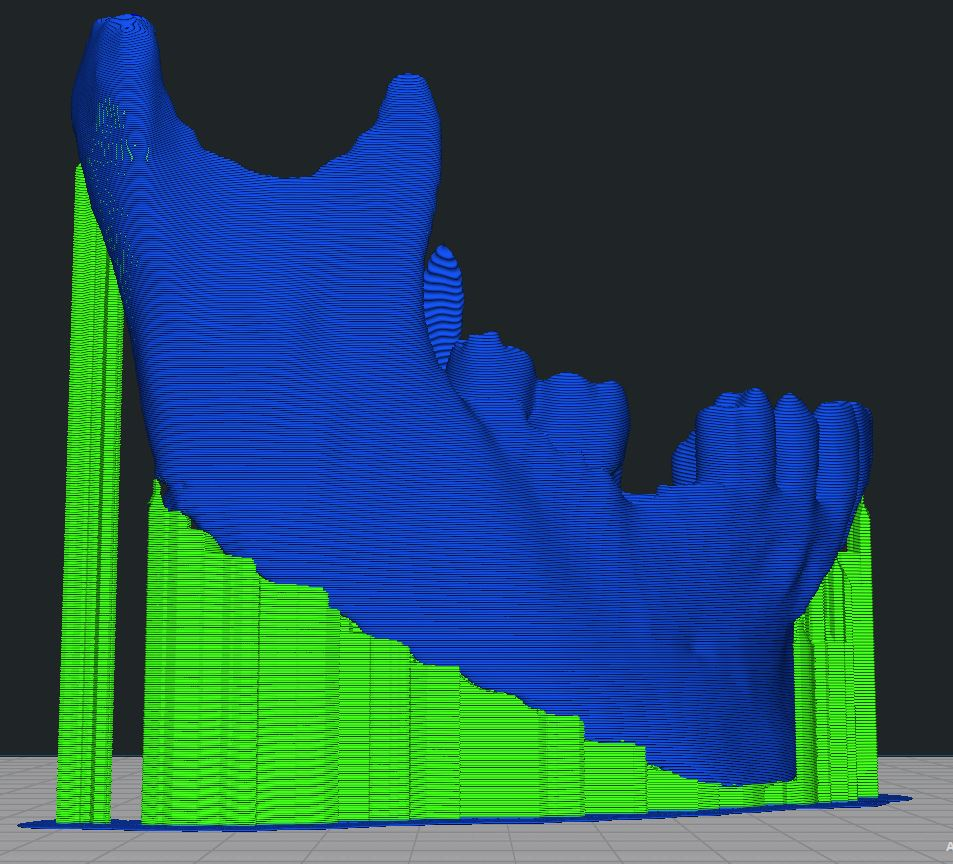
\includegraphics[width=0.5\textwidth, height=\textheight,keepaspectratio]{Supports}
    \caption{Supporti in verde}
    \label{fig:Supports}
\end{figure}

	
\subsection{Build Plate Adesion}
Il menù \emph{\textbf{Build Plate Adesion}} permette di generare dei contorni o superfici per favorire l'adesione del primo strato dell'oggetto al piano.\\

\textbf{Skirt} è semplicemente un giro che di estrusione compiuto attorno al perimetro del modello da stampare, senza toccarlo; serve al priming dell'estrusore, ciò ad estrudere del materiale prima della stampa in modo che l'ugello sia pronto per iniziare il primo strato.\\

\textbf{Brim} è un contorno che si congiunge al margine del primo strato dell'oggetto. Se ne può regolare l'ampiezza ed è un aiuto importante nel mantenere i modelli aderenti al piano. È anche facile da rimuove e non lascia praticamente segni sul modello.\\

\textbf{Raft} è una griglia spessa pochi layers, prodotta tra il piano e l'oggetto. Raft migliora l'adesione anche su una superficie non regolare e permette una buona distribuzione del calore al modello. Utile per stampare materiali che si deformano molto in seguito al processo di stampa.
\begin{figure}[h]
 
\begin{subfigure}{0.5\textwidth}
\centering
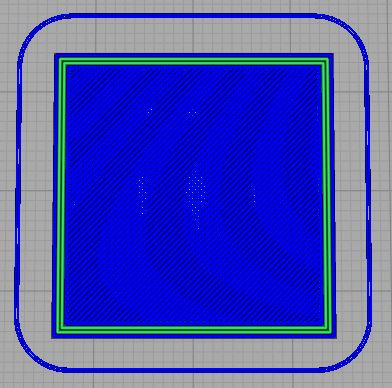
\includegraphics[width=0.7\linewidth, keepaspectratio]{skirt} 
\caption{Skirt}
\label{fig:skirt}
\end{subfigure}
\begin{subfigure}{0.5\textwidth}
\centering
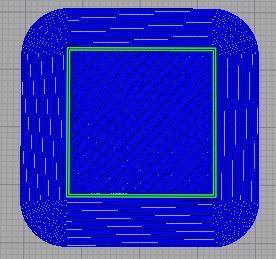
\includegraphics[width=0.7\linewidth, keepaspectratio]{brim}
\caption{Brim}
\label{fig:brim}
\end{subfigure}
\begin{subfigure}{0.5\textwidth}
\centering
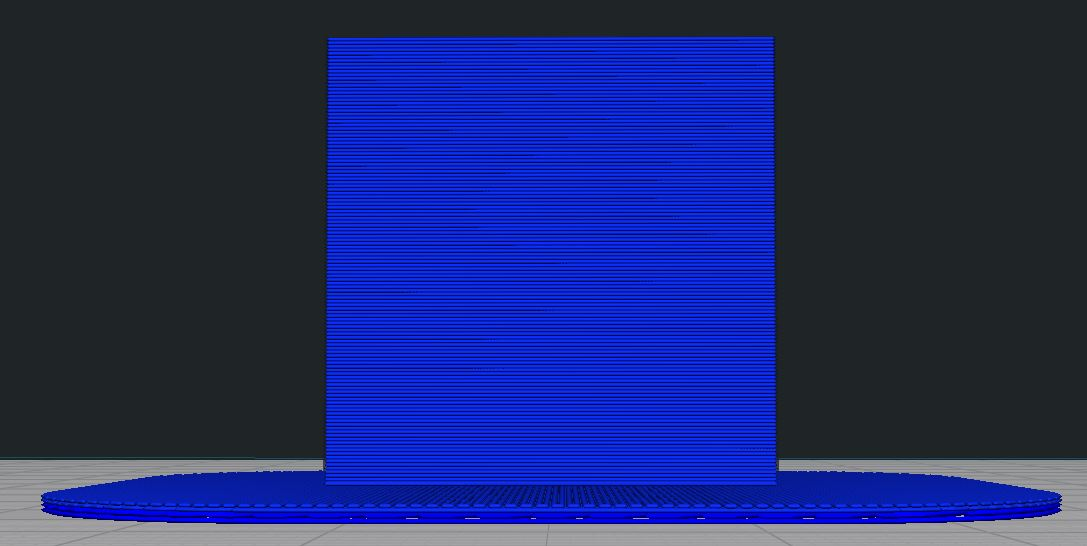
\includegraphics[width=0.9\linewidth, keepaspectratio]{raft}
\caption{Raft}
\label{fig:raft}
\end{subfigure}
 
\caption{Opzioni delle basi di adesione in \emph{Build Plate Adesion}.}
\label{fig:Build Plate Adesion}
\end{figure}

\subsection{Fixes, Special Modes ed Experimentals}
Gli altri menù contengono altri controlli avanzati sulla riparazione della mesh durante la stampa, modalità di stampa speciali e funzioni sperimentali, che non sono fondamentali per le procedure qui descritte, ma che vale comunque la pena conoscere, perche utili in alcuni frangenti.\\
Il \emph{\textbf{Special Modes}} troviamo l'opzione \emph{Print Sequence} da la possibilità di stampare gli oggetti sul piano tutti insieme oppure uno alla volta. \\
L'opzione \emph{Mold} da la possibilità di creare dei negativi del modello, che possono essere stampati ed utilizzati per ricreare il modello che era originariamente sul piano.\\
In \emph{\textbf{Experimental}}, la voce \emph{slicing tollerance} indica come si deve effettuare lo slicing delle superfici diagonali e ne influenza la modalità di slicing \parencite{Reference56}. Importante per gestire la tolleranza di componenti meccaniche che necessitano di una adeguata precisione.
